\section{Trigonometrie}
	\subsection{Geometrische Trigonometrie}
	Das Thema Trigonometrie in der Geometrie umfasst eine Reihe an verschiedenen Unterthemen. Hierbei
spielt das rechtwinkelige Dreieck eine wesentliche Rolle und bestimmt somit auch die Wurzeln der
Trigonometrie. Bei der geometrischen Trigonometrie geht es vorwiegend um das Bestimmen von
Seitenlängen oder Winkeln.
\begin{center}
	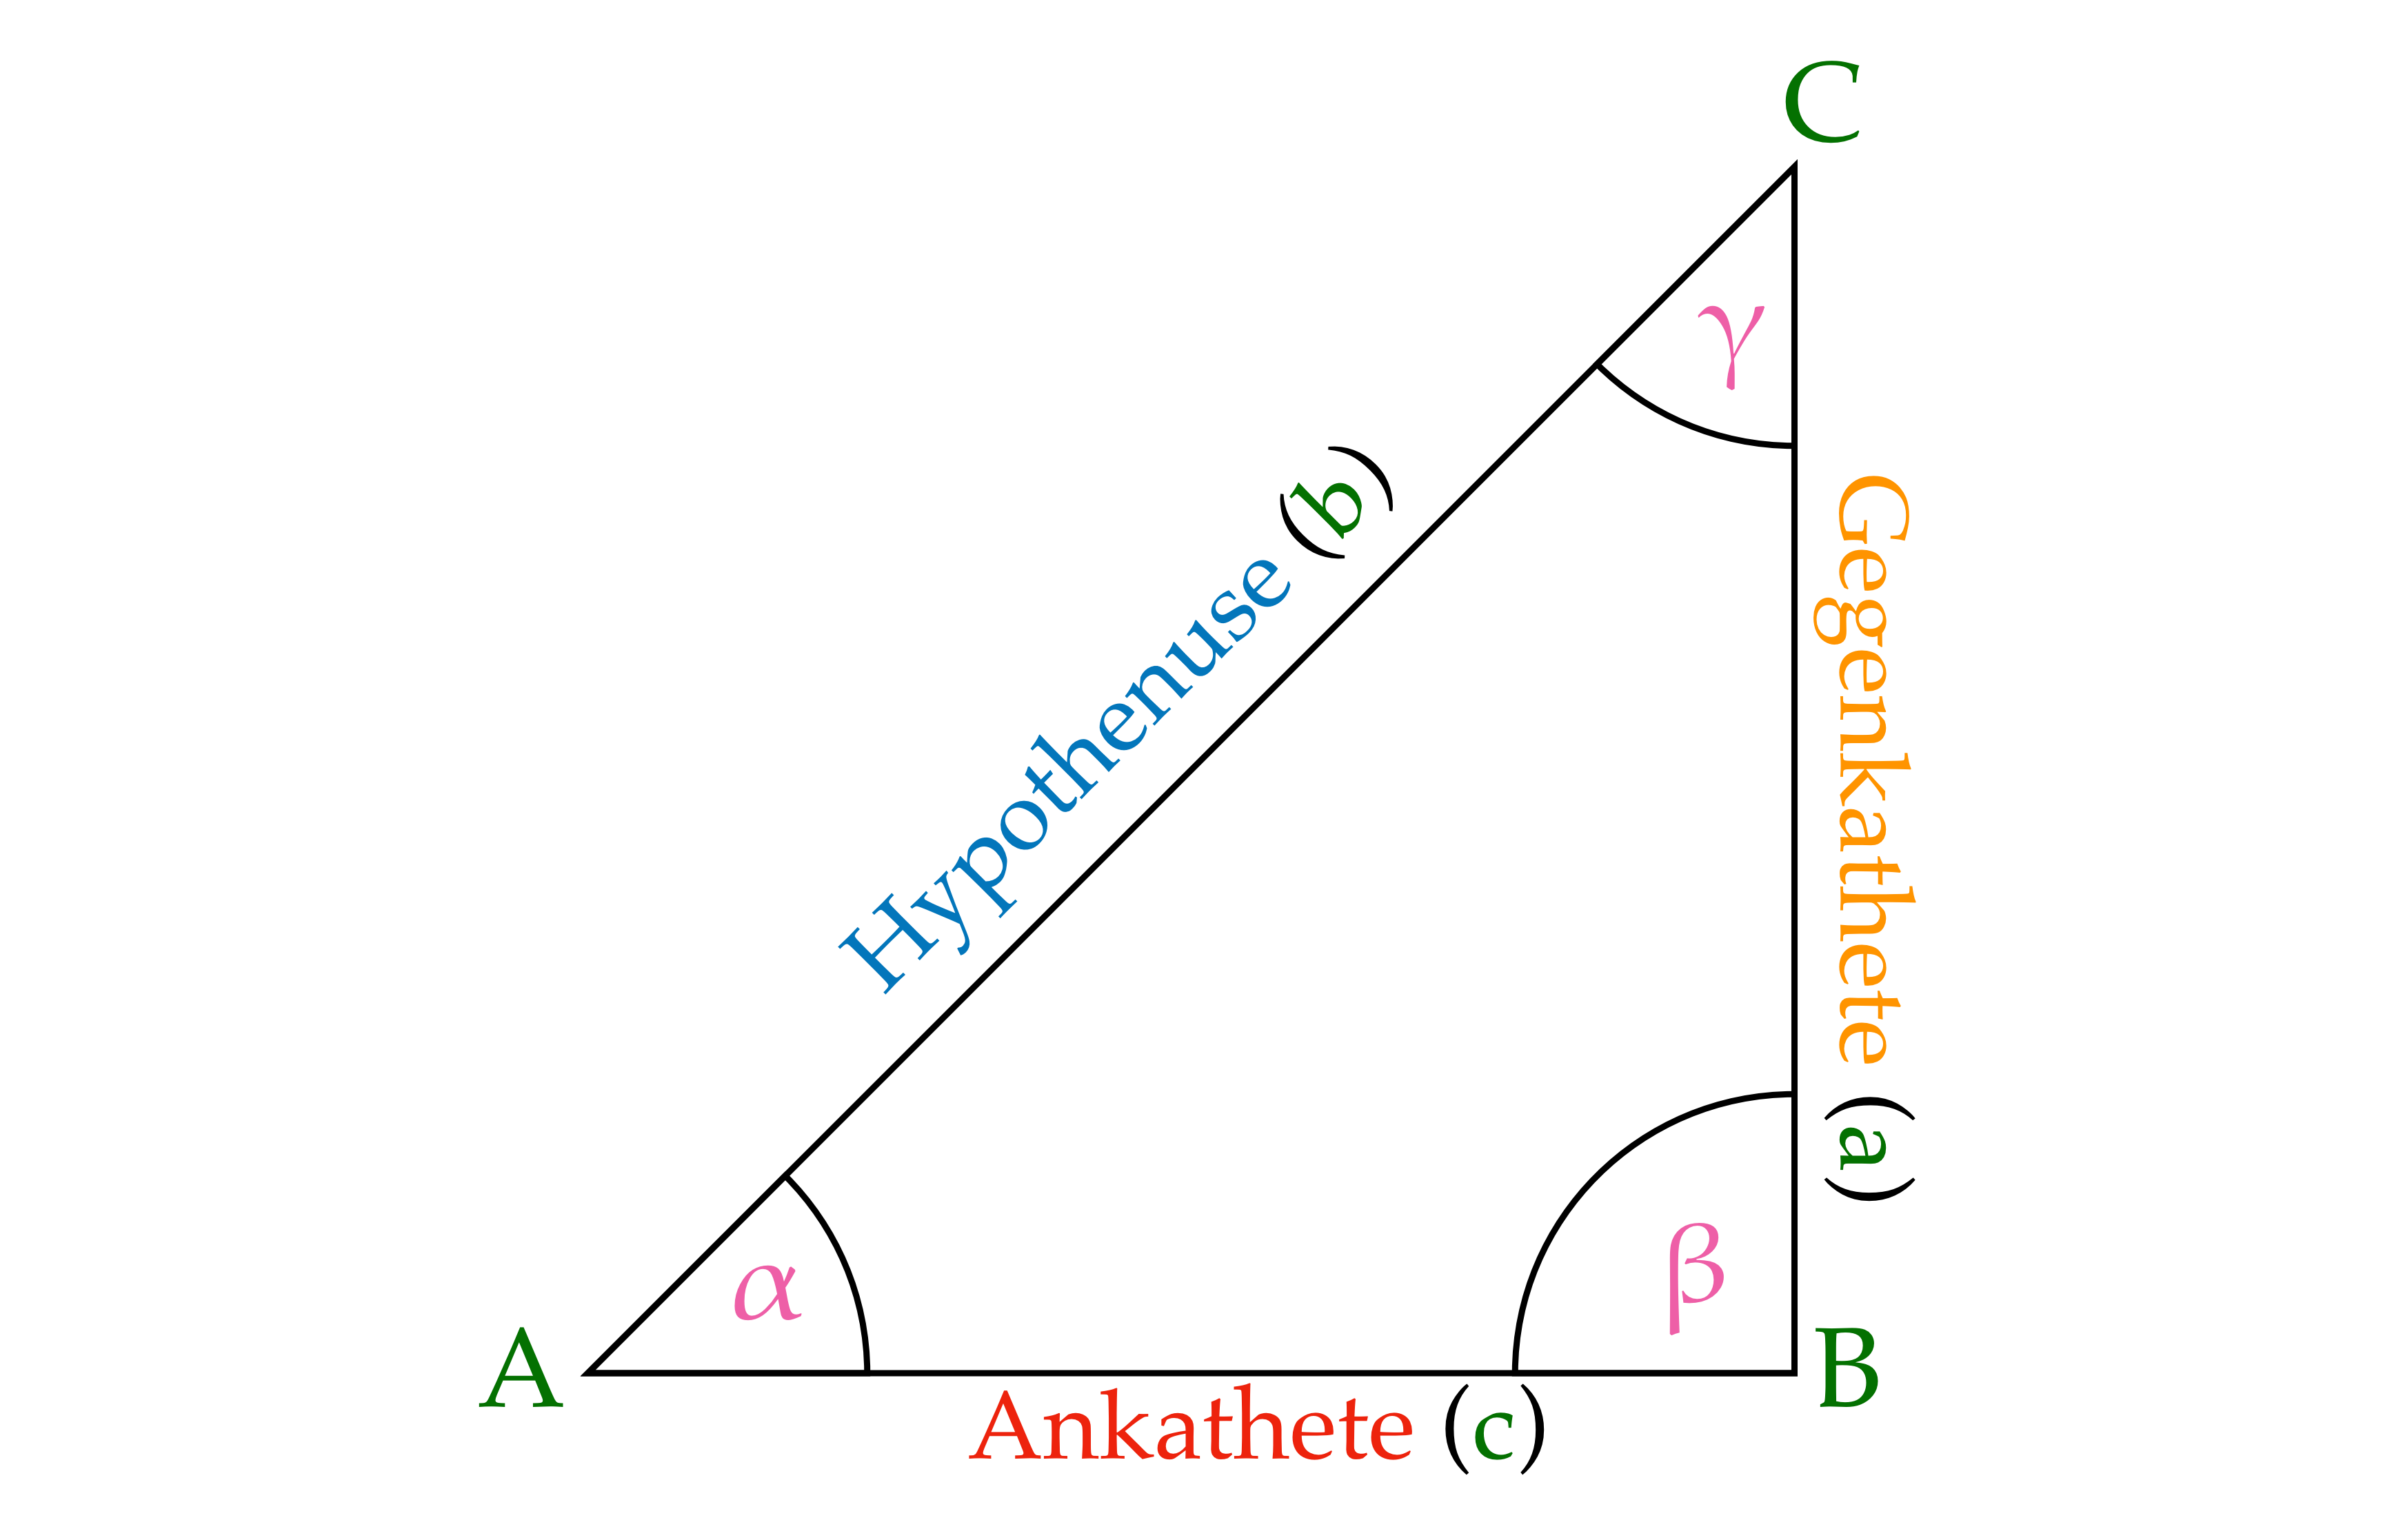
\includegraphics[width=200pt, height=130pt]{Media/Dreieck}
\end{center}
\begin{itemize}
	\item[\textcolor{darkgreen}{\textbf{A, B, C}}]{}
	Die Ecken eines rechtwinkeligen Dreiecks sind mit großen Buchstaben gekennzeichnet
	
	\item[\textcolor{darkgreen}{\textbf{a,b,c}}]{Die gegenüberliegenden Seiten sind mit dem jeweils
	gleichen Buchstab in klein gekennzeichnet
	Stellen jeweils die Winkel zwischen den anliegenden Seiten dar und ergeben zusammen 180 Grad.
	Die Gegenkathete stellt die Höhe
	des Dreiecks dar, während die Ankathete die Seite ist, die am rechten Winkel  und  anliegt}
	
	
	\item[\textcolor{blue}{\textbf{Hypothenuse}}]{}
	Die Hypothenuse stellt im Dreieck die Seite $b$ dar. Sie ist die längste Seite und immer
	gegenübervon rechten Winkel, wobei sie nie an ihm anliegt. 


	\item[\textcolor{red}{\textbf{Ankathete}}]{}
	Die Ankathete ist die Seite $c$ in einem Dreieck und liegt immer am rechten Winkel an. Sie bildet mit der Gegenkathete den rechten Winkel und ist hierbei immer kürzer als die Hypothenuse
	
	
	\item[\textcolor{orange}{\textbf{Gegenkathete}}]{}
	Die Gegenkathete beschreibt in einem Dreieck die Seite a und liegt direkt an dem rechten Winkel,
	den sie mit der Ankathete bildet. 
\end{itemize}
\pagebreak

% Neue Seite ################################################################################################################################################
\subsection{Berechnung der Seiten und des Winkels}
	Um eine Berechnung der Seiten durchführen zu können, muss verwendet man folgende Formeln:\\
	\\
	
\textbf{Sinus} \[ \sin(\alpha)=\frac{Gegenkathete}{Hypotenuse} \]
\textbf{Cosinus} \[ \cos(\alpha)=\frac{Ankathete}{Hypothenuse} \]
\textbf{Tangens} \[ \tan(\alpha)=\frac{Gegenkathete}{Ankathete} \]
\\
\\
Um einen ersten Anhaltspunkt zu schaffen, kann man sich an dem folgenden Algorythmus orientieren. 


\includegraphics[width=15cm]{Media/Algorythmus_Berechnung_eines_Dreiecks}



\pagebreak
% Neue Seite ################################################################################################################################################

\subsection{Trigonometrische Funktionen}
 	Auch in der Analyses spielt die Trigonometrie einen wichtige Rolle. Sie ermöglicht es periodische Prozesse darzustellen und mit ihnen zu rechnen. So lassen sich Sinus, Cosinus und Tangens jeweils im Koordinatensystem herleiten am Einheitskreis.

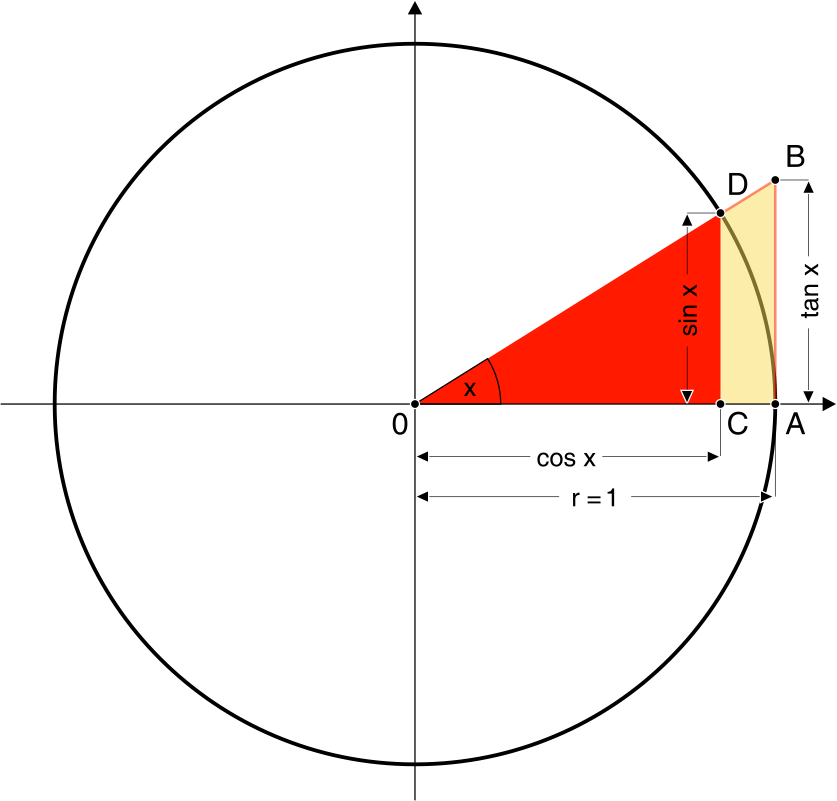
\includegraphics[width=10cm]{Media/Winkelfunktionen_Einheitskreis}\\
So stellt Sinus die Höhe der Gegenkathete in Abhängigkeit von dem Bogenmass, welches mit Hilfe des
Winkels Alpha berechnet wird. Cosinus hingegen stellt die Ankathete in Abhängigkeit des Bogenmasses dar. Hierbei orientieren sich die Eckpunkt jeweils an dem Einheitskreis und laufen auf 
diesem gegen den Uhrzeigersinn. Hierdurch entsteht die wellenförmige Ausprägung des Graphen. Da Sinus die Höhe der Gegenkathete darstellt in Abhängigkeit von dem Bogenmass befindet sich die
dargestellte Höhe der Gegenkathete auf einer Höhe von $\pi$ auf der X-Achse. 
\\
\\
\textbf{Begründung der Periodenlänge}
Durch den Einheitskreis wird die Perioden länge bestimmt, da das Bogenmass auf der X-Achse dargestellt wird. So ist eine halbe Umrundung des Kreises genau ein $\pi$ lang. 


\subsection{Überleitung zu trigonmetrische Funktionen}
Aufgrund der Veränderung der verschiedenen Seitenlängen des rechtwinkeligen Dreiecks, welche durch die jeweilge trigonometrische Funktion dargestellt wird und abhängi
von dem Winkel $\alpha$ ist, entsteht die pregnante Form von Sinus und Cosinus. 
\\
%\link{https://de.wikipedia.org/wiki/Trigonometrische_Funktion#/media/Datei:Circle_cos_sin.gif}{Veranschaulichung Entstehung von Sinus Cosinus}


\subsection{Normalform einer trigonometrischen Funktion}
Ähnlich wie quadratische Funktionen oder lineare Funktionen gibt es ebenfalls einen Normalform der Sinus Funktion.
\[a\cdot sin(b(x+d))+e\]
\\
$a$: Streckfaktor auf der X-Achse(Amplitude) \\
$b$: Streckfaktor auf der Y-Achse (Periodenlänge)\\
$d$: Verschiebung auf der X-Achse\\
$e$: Verschiebung auf der Y-Achse \\
	\pagebreak
	
% Neue Seite ################################################################################################################################################
\subsection{Moddelierung der Sinus Funktion}
Für die Moddelierung einer Sinus oder Cosinus Funktion kann man wie folgt vorgehen.

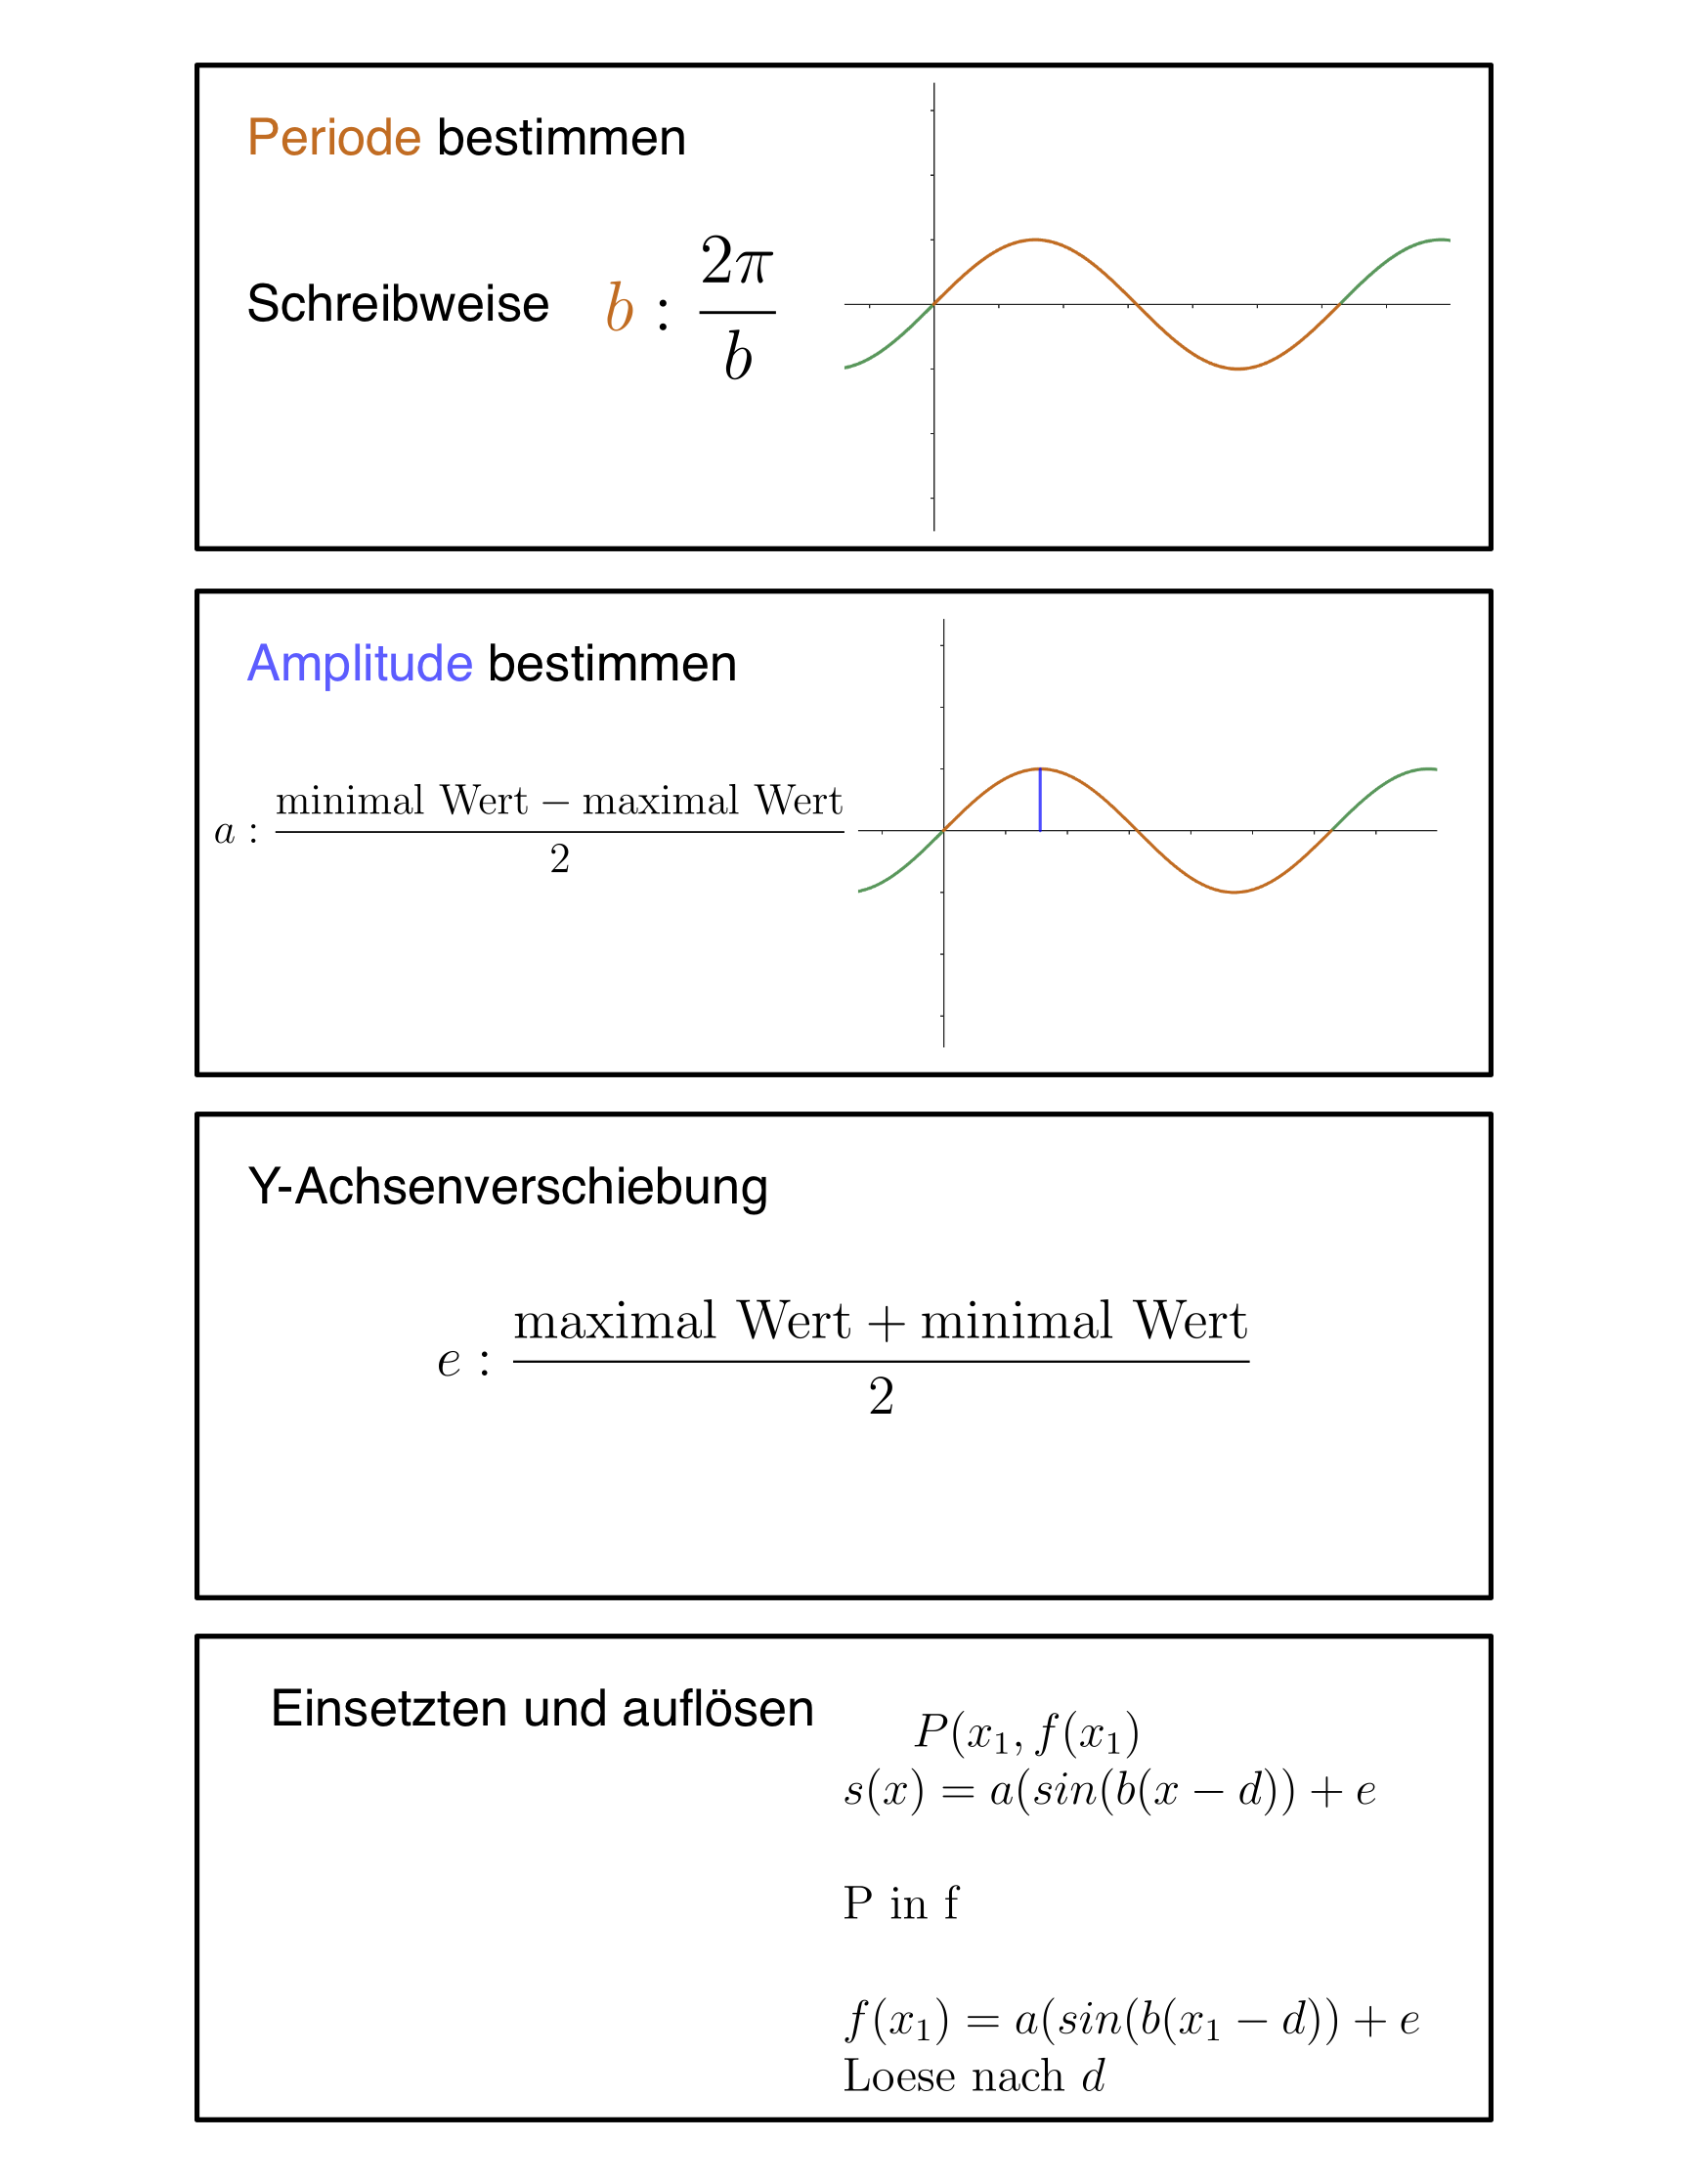
\includegraphics[width=13cm]{Media/Modelierung_von_Sinus_Algorythmus}

